\subsection{Feasibility study}

\begin{frame}{Jets \pt}
\vspace{-.4cm}
\begin{figure}[!Hhtbp]
  \begin{center}
    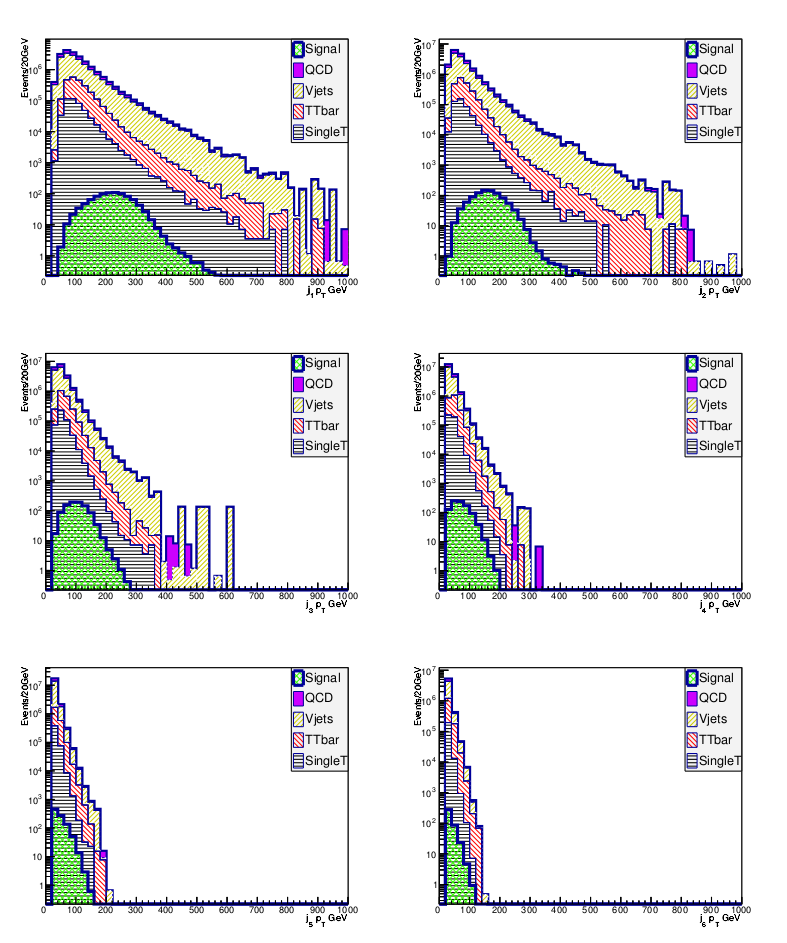
\includegraphics[width=0.55\textwidth]{../figs/Pheno/JetPt.png}
    %\caption{$p_{T}$  of the six leading jets for backgrounds (stacked) and signal (over--imposed) normalized to 20 $fb^{-1}$ luminosity. QCD background is on top of the stack of backgrounds.}
    %\label{fig:Var1}
  \end{center}
\end{figure}
\vspace{-.4cm}
    \begin{block}{}
      \tiny \centering $p_{T}$  of the six leading jets for backgrounds (stacked) and signal (over--imposed) normalized to 20 $fb^{-1}$ luminosity. QCD background is on top of the stack of backgrounds.
    \end{block}

\end{frame}

\begin{frame}{B-jet multiplicity requirement}
\vspace{-.2cm}
\begin{figure}[!Hhtbp]
  \begin{center}
    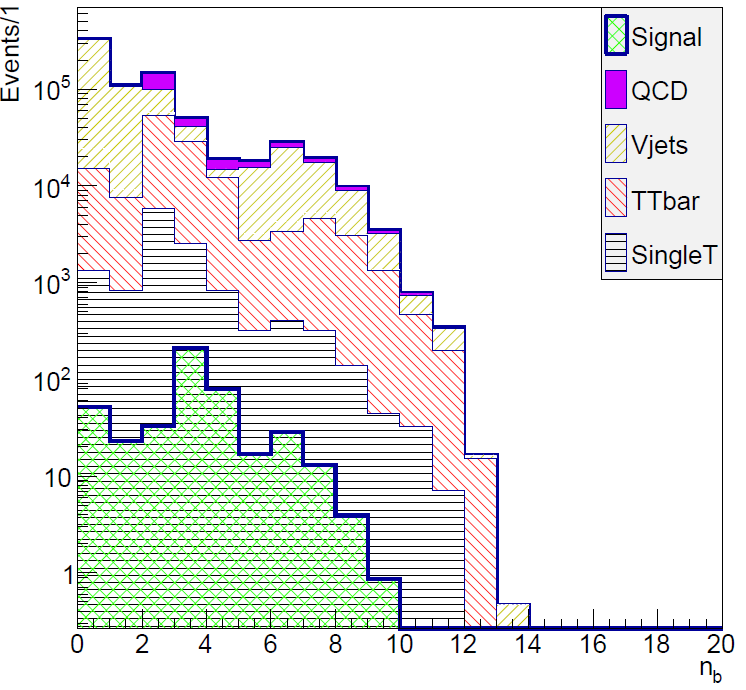
\includegraphics[width=0.45\textwidth]{../figs/Pheno/Nb.png}
    %\caption{B-tagged jet multiplicity for backgrounds (stacked) and signal (over--imposed) normalized to 20~$fb^{-1}$ luminosity. The signal has as mean value 3 b-tagged jets.}
    %\label{fig:Nbs}
  \end{center}
\end{figure}

\vspace{-.2cm}
    \begin{block}{}
      \tiny B-tagged jet multiplicity for backgrounds (stacked) and signal (over--imposed) normalized to 20~$fb^{-1}$ luminosity. The signal has as mean value 3 b-tagged jets. The following method was used to emulate the performance of b-jet identification algorithms:
  \begin{enumerate}\tiny
  \item The CMS results for CSVM were used: $\epsilon^{b-tag}_{b}=0.9$, $\epsilon^{b-tag}_{c}=0.6$ and $\epsilon^{b-tag}_{l}=0.1$.
  \item Throw a random number $r$ between 0 and 1 for each event.
  \item Loop over all the jets from an event and, depending on their flavor and the random number from last step, declare each jet to be or not to be b-tagged. A jet is b-tagged if: it is coming from a b-quark and $r\leq\epsilon^{b-tag}_{b}$, or it is coming from a c-quark and $r\leq\epsilon^{b-tag}_{c}$, or it is coming from a light-quark and $r\leq\epsilon^{b-tag}_{l}$.
  \end{enumerate}
    \end{block}

\end{frame}

\begin{frame}{}
\vspace{-.2cm}

\vspace{-.2cm}
    \begin{block}{}
      \tiny \centering 
    \end{block}

\end{frame}

\begin{frame}{}
\vspace{-.2cm}

\vspace{-.2cm}
    \begin{block}{}
      \tiny \centering 
    \end{block}

\end{frame}

\begin{frame}{}
\vspace{-.2cm}

\vspace{-.2cm}
    \begin{block}{}
      \tiny \centering 
    \end{block}

\end{frame}

\begin{frame}{}
\vspace{-.2cm}

\vspace{-.2cm}
    \begin{block}{}
      \tiny \centering 
    \end{block}

\end{frame}

\begin{frame}{}
\vspace{-.2cm}

\vspace{-.2cm}
    \begin{block}{}
      \tiny \centering 
    \end{block}

\end{frame}